\section{Related Work}
\subsection{Autoregressive Image Generation}
Autoregressive (AR) models have shown powerful generation ability across modalities~\cite{Flamingo, Videollava, llavamed, Unifiedio2}, and their extension to visual generation~\cite{ImageTransformer, llamagen, Chameleon, Emu, Emu3, januspro, simpleAR} has demonstrated promising potential. Typically, they follow a two-stage paradigm: a tokenizer encodes images into discrete representations (e.g., VQ-VAEs~\cite{VQ_VAE, VQ_VAE2}, RQ-VAE~\cite{RQ_VAE_RQ_FORMER}, VQ-GAN~\cite{VQ_GAN, VIT_VQGAN}), and a transformer decoder~\cite{MaskGIT, star_scale_wise, VAR, RAR, SpectralAR} that sequentially predicts these tokens for image reconstruction.

Most AR models use 2D patch-wise tokenization, capturing local details but lacking holistic awareness~\cite{MVTQ, EfficientVQGAN, ARPG_LocalTokens, ImageGPT}. To improve global coherence, recent works explore complementary strategies: global-context modeling~\cite{Hita} introduces holistic queries for structural reasoning; frequency-domain methods~\cite{SpectralAR, NFIG} encode coarse-to-fine spectral context; 1D tokenizers~\cite{Titok, FlexTok, InstellaT2I} enhance efficiency but lose adaptability; semantic tokenization~\cite{ImageFolder, TexTok} leverages language priors for meaningful visual codes. Structured visual like glyphs, however, demands tokenizers that unify local stroke detail with global aesthetics. Our GAR-Font addresses this challenge through a \textbf{global-aware tokenizer} that integrates CNN-based locality with Transformer-based global reasoning, effectively unifying fine-grained stroke detail and overall stylistic coherence.

\subsection{Few-shot Font Generation}
Few-shot Font Generation (FFG) can be broadly divided into vector-based and image-based approaches. Vector FFG methods have progressed in sequential modeling and efficient representations~\cite{FontRNN, Deepvecfont, DeepVecFontV2, DualVector, Vecfusion, Vecfontsdf}. Yet complex ideographic generation and unseen glyph generalization remain challenging~\cite{EasyFont, CVFont}. Image-based methods, in contrast, learn 2D pixel priors for robust adaptation, evolving from early image-to-image translation~\cite{zi2zi, word2word, zigan, HGAN} to more recent VQ and diffusion formulations~\cite{Font_Diffuser, HFH_Font, FSTDIFF, VQ_Font}. These models typically employ content–style disentanglement to separately capture structure and style~\cite{zhang2018separating, EMD, AGIS-Net, DG_Font, MX_Font, DS-Font, FineGrainedFFG, fewshotFFG, Xmpfont, Diff_Font}, enhanced by mechanisms like contrastive learning for global coherence~\cite{SCFont} and cross-attention for local transfer~\cite{Fs_Font}.  

The challenge is most acute for glyph-rich, ideographic languages such as Chinese and Korean, where thousands of characters demand fine structure and faithful global style~\cite{LegacyLearning, SCFont, GenerateExpert, HFH_Font}. In this regime, \textbf{image-based AR models that operate FFG on globally contextualized visual tokens} show particular promise: by modeling spatial dependencies directly in the 2D domain, they better capture the intricate geometry and visual regularities of glyphs.

\begin{figure}[t!]
    \centering
    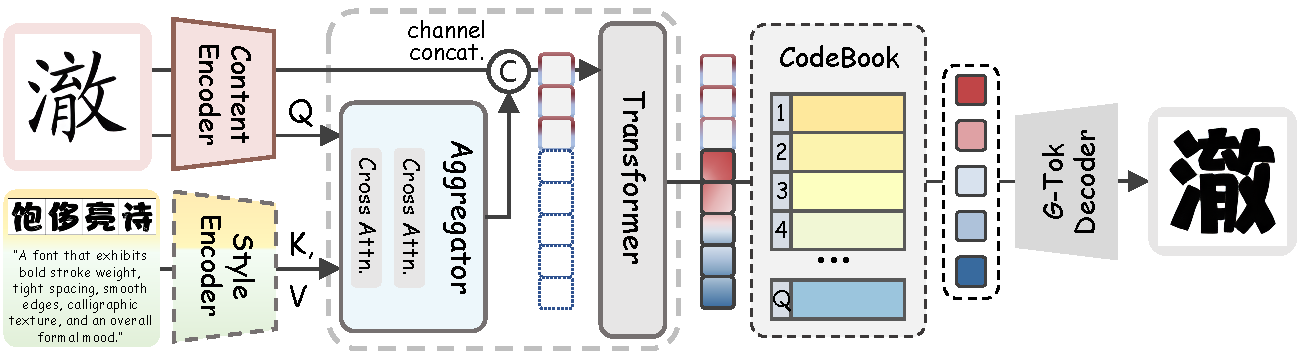
\includegraphics[width=\linewidth]{IMGS/Fig1_Model.pdf}
    \vspace{-4mm}
    \caption{The overall architecture of GAR-Font. It comprises a global-aware tokenizer (G-Tok), and an AR generator, equipped with a multimodal style encoder.}
    \vspace{-3mm}
    \label{fig: Model}
\end{figure}
\begin{figure*}[!t]
\centering
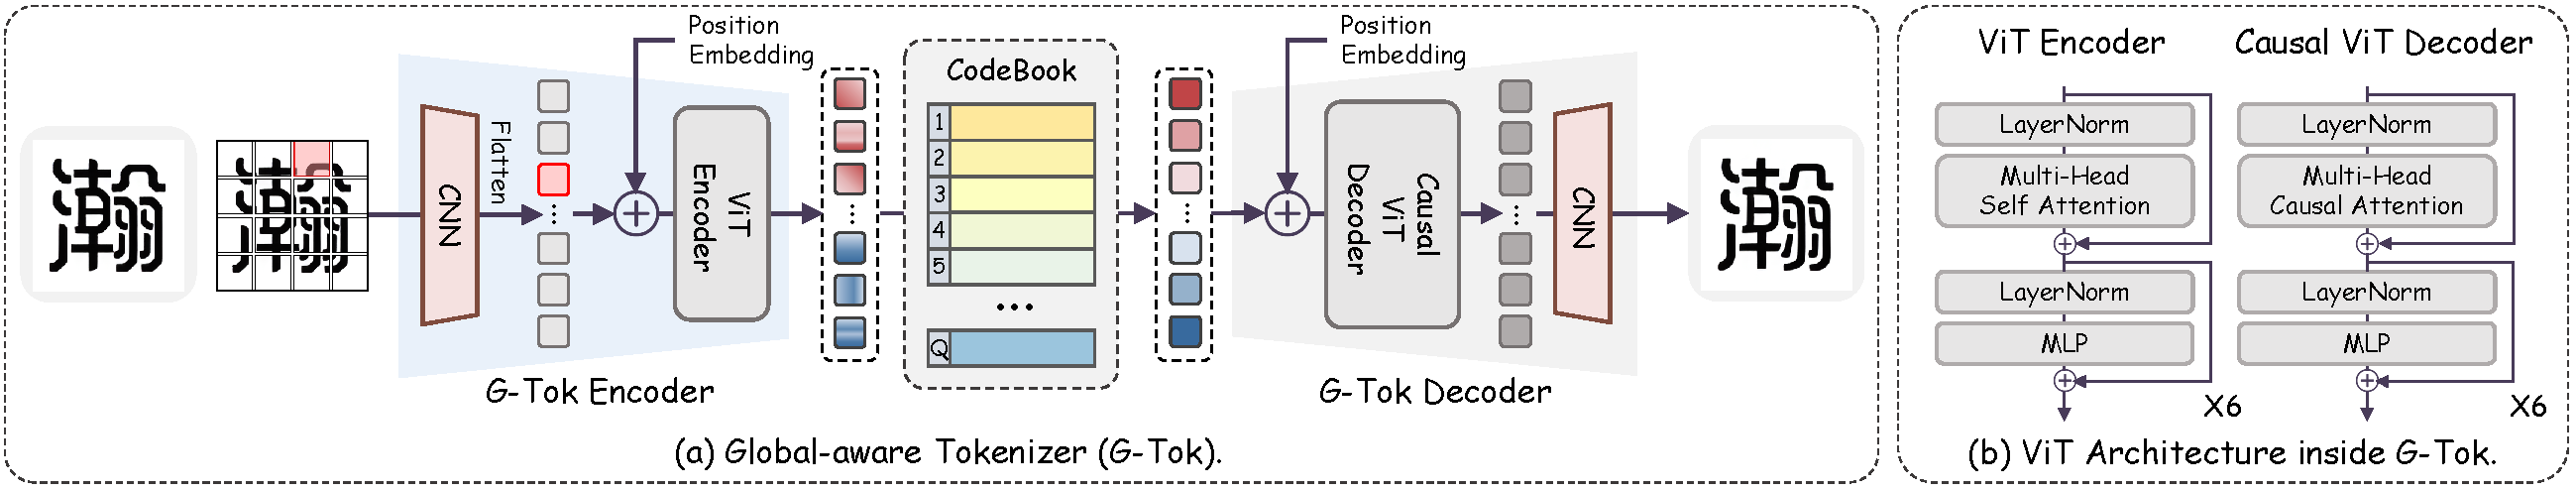
\includegraphics[width=0.99\linewidth]{IMGS/Fig2_G-Tok.pdf}
\vspace{-3mm}
\caption{(a) Overview of the G-Tok architecture, which adopts a hybrid CNN–ViT design. (b) Details of the global ViT encoder and causal ViT decoder. With self- and causal-attention, G-Tok captures global dependencies, enabling coherent and high-quality font synthesis.}
\vspace{-3mm}
\label{fig: G-tok}
\end{figure*}
\subsection{Multimodal Alignment for Style Control}
Multimodal alignment for style control unifies visual and textual modalities for coherent, fine-grained style manipulation. Foundational models~\cite{Emu3, januspro, BAGEL, Seed-X, Qwen-Image, Hunyuan-Image} achieve this through costly multimodal pretraining. For fonts, however, only textual inputs describing style are incorporated, and the independent encoding of content and style in FFG frameworks~\cite{VQ_Font, Fs_Font, LF_Font} naturally forms a structured visual style space that serves as a strong prior for multimodal integration. Recent works pursue efficient alignment via parameter-efficient modules~\cite{FonTS, FontAdapter, LoRA, AdaCLIP} or resampler-based strategies aligning vision and language spaces~\cite{Flamingo, PaLM2-VAdapter, CalliReader, TextAdapter}. Motivated by these works, GAR-Font extends the style encoder in FFG models to a \textbf{multimodal style encoder} that consists of a visual style encoder and a lightweight pluggable \textbf{language-style adapter} that aligns textual descriptions with visual style embeddings, enabling fine-grained, flexible style control without the need for large-scale multimodal pretraining.
